\documentclass[10pt,a4paper]{article}
\usepackage[margin=2.2cm]{geometry}
\usepackage{fontspec}
\usepackage{kotex}
\setmainfont{Apple SD Gothic Neo}
\setsansfont{Apple SD Gothic Neo}
\usepackage{amsmath,amssymb}
\usepackage{graphicx}
\usepackage{booktabs}
\usepackage{caption}
\usepackage[dvipsnames]{xcolor}
\usepackage[colorlinks=true,linkcolor=MidnightBlue,citecolor=MidnightBlue,
            urlcolor=MidnightBlue]{hyperref}
\usepackage{titlesec}
\titleformat{\section}{\large\bfseries}{\thesection}{0.6em}{}
\titleformat{\subsection}{\normalsize\bfseries}{\thesubsection}{0.5em}{}
\captionsetup{font=small,labelfont=bf}
\setlength{\parskip}{0.35em}
\setlength{\parindent}{0pt}

\usepackage{mdframed}
\newmdenv[linewidth=0.4pt,linecolor=gray!60,backgroundcolor=gray!5,
          innertopmargin=6pt,innerbottommargin=6pt,skipabove=8pt,skipbelow=8pt]{claimbox}
\newcommand{\claim}[2]{\begin{claimbox}\textbf{주장.} #1\par\smallskip
  \textcolor{gray!70}{\textbf{반증 조건.} #2}\end{claimbox}}

\title{\bfseries 고르기가 상쇄를 못 이긴다\\[2pt]
\large 짝 단위 이득은 실재하는데 그것으로 소스를 고르면 위약보다 나빠진다 --- 트랙을 닫는다}
\author{월드모델 실험실 · 노트 728 · 729 · 730 · 731 (T5 종결)}
\date{2026-08-06}
\begin{document}\maketitle

\section{한 줄}

논문 143 이 \emph{``설계 물음이 무엇을 같이 학습하나에서 무엇을 소스로
쓰나로 바뀐다''}로 끝났고, 논문 142 계열의 짝 행렬이 \textbf{문턱의 $19.5$배
짝}(웹툰$\to$애니 $+0.207$)을 실제로 찾았다. 그래서 \textbf{목표마다 도움이 되는
소스만 골라} 트렁크를 적합했다. \textbf{판 신호 몫이 $\mathbf{-0.0027}$ 이다} ---
문턱 밖은커녕 \textbf{값을 섞은 위약보다 나쁘다.} 이것이 T5(아키텍처)의 세 번째이자
마지막 문이었고, \textbf{트랙을 닫는다.}

\section{왜 될 것 같았나 --- 반증당한 것은 내 예측이다}

\textbf{사전등록 예측은 $0.008 \sim 0.018$} 이었다(``조금 오르지만 결정적이지
않다''). 근거 셋을 적었다: ① 짝 행렬에 문턱의 $20$배 짝이 여럿 있다 ② 전부 합치면
큰 양수와 큰 음수가 상쇄되므로 고르면 그 상쇄가 풀린다 ③ 아이돌처럼 크게 해로운
소스를 빼는 것만으로 얼마간 오른다.

\begin{center}
\begin{tabular}{lrr}
\toprule
& 사전등록 & \textbf{실측} \\
\midrule
판 신호 몫(진짜 $-$ 위약) & $+0.008 \sim +0.018$ & $\mathbf{-0.0027}$ \\
노트 721 의 $+0.0106$ 초과 & 예 & \textbf{아니오} \\
문턱 $0.0045$($2\sigma$) 밖 & 예 & \textbf{아니오} \\
시장팝업 도메인을 뺀 판 & 그래도 양수 & $+0.0019$ (\textbf{역시 미달}) \\
\bottomrule
\end{tabular}
\end{center}

세 판정이 다 실패했고 \textbf{사전등록의 틀림 조건 ②가 발동했다} ---
\emph{``$+0.0045$ 미달이면 소스 고르기도 안 되는 것이고 T5 를 닫는다.''}

\subsection*{누출은 막았다 --- 그것이 이 실험의 주제였다}

노트 727 이 스스로 경고를 적었다: \emph{``소스를 고르는 것 자체가 유보를 보고 고르는
것이면 누출이다.''} 그래서 구간을 셋으로 갈랐다.

\begin{center}
\begin{tabular}{ll}
\toprule
\textbf{앞} ($<2024$) & 소스별 트렁크를 적합한다 \\
\textbf{뒤} ($2024$) & 그 트렁크로 목표를 채점해 \textbf{행렬을 만든다} \\
\textbf{유보} ($\geq 2025$) & \textbf{소스 고르기에 한 번도 쓰지 않는다} \\
\bottomrule
\end{tabular}
\end{center}

\begin{figure}[t]\centering
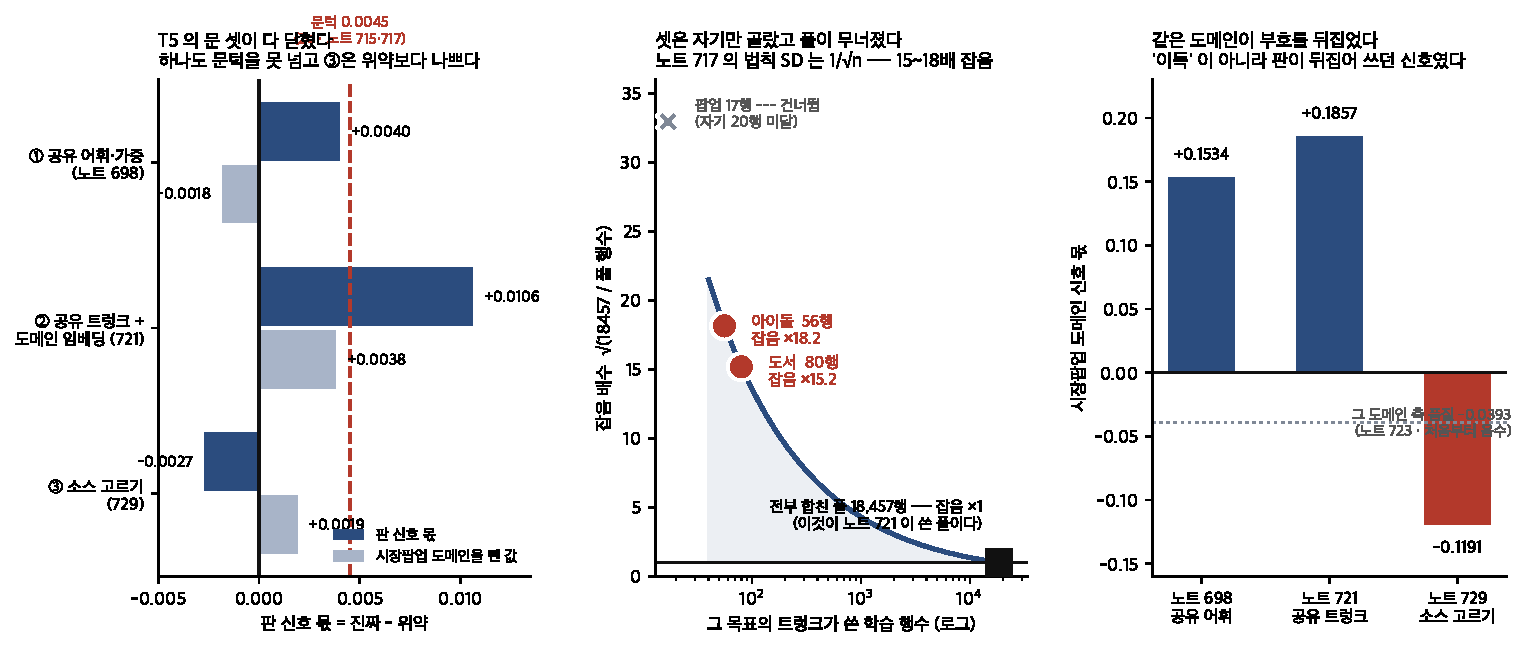
\includegraphics[width=0.99\textwidth]{figs/shrinkpool.pdf}
\caption{왼쪽: \textbf{T5 의 문 셋이 다 닫혔다} --- 셋 중 하나도 문턱($2\sigma$)을 못
넘고 ③은 음수다(위약보다 나쁘다). 가운데: \textbf{셋은 자기만 골라 풀이 무너졌다} --- 노트 717 의
$\text{SD} \propto 1/\sqrt{n}$ 이 잡음을 $15{\sim}18$배로 매긴다. 오른쪽:
\textbf{시장팝업이 부호를 뒤집었다.}}
\end{figure}

\section{왜 해로웠나 --- 원인 둘을 적었는데 하나의 사슬이었다}

\subsection*{하나: 풀을 줄이는 비용이 고르기 이득보다 크다}

목표마다 고른 소스 수가 세계애니 $8$ · 애니 $7$ · 모바일 $6$ · 펀딩 $6$ · 게임 $5$ ·
만화 $4$ · 시장팝업 $4$ · 웹툰 $3$ 인데, \textbf{도서 · 아이돌 · 팝업 셋은 자기만
골랐다} --- 양수 소스가 하나도 없었다는 뜻이다.

\begin{center}
\begin{tabular}{lrrr}
\toprule
목표 & 그 트렁크가 쓴 학습행 & 전부 대비 & \textbf{잡음 배수} \\
\midrule
전부 합친 풀 (노트 721) & $18{,}457$ & $1\times$ & $\times 1.0$ \\
\midrule
도서 & $80$ & $1/231$ & $\mathbf{\times 15.2}$ \\
아이돌 & $56$ & $1/330$ & $\mathbf{\times 18.2}$ \\
팝업 & $17$ & $1/1086$ & 건너뜀(자기 $20$행 미달) \\
\bottomrule
\end{tabular}
\end{center}

노트 717 이 \textbf{잡음의 참값 $0$ 표준편차가 $c/\sqrt{n}$} 임을 쟀다. 그 법칙이
여기 값을 매긴다 --- \textbf{풀이 $231$배 작아지면 그 트렁크의 예보 잡음이 $15$배
커진다.} 짝 하나의 이득이 그만큼 크지 않다.

\claim{\textbf{소스 고르기는 잡음 예산 안에서만 이득이다.} 고르기는 상쇄를 푸는
대신 풀을 줄이고, 풀 축소는 $1/\sqrt{n}$ 으로 값을 물린다. \textbf{그러므로 ``어떤
소스가 도움이 되나''를 알아도 그것을 쓰려면 도움 되는 소스가 \emph{충분히 많아야}
한다} --- 열한 도메인 중 셋은 하나도 없었다.}
{도움 소스가 적은 목표에서 \textbf{전부 합친 풀로 되돌리는} 혼합 규칙(고르기와 전부
사이 축소 추정)을 쓰면 이 비용을 피할 수 있다. 그 규칙으로도 문턱을 못 넘으면 이
주장이 아니라 ``짝 이득 자체가 없다''가 맞다. \textbf{다만 그 실험은 안 돌렸다} ---
아래에서 이 원인이 \emph{독립 원인이 아니라} 둘째 원인의 결과임이 드러난다.}

\subsection*{둘: 고를 근거가 절반쯤 잡음이었다 --- 그리고 원인 둘이 하나의 사슬이었다}

초고에서 나는 \emph{``두 행렬이 같은 소스를 고르지 않는다''}고 \textbf{단정했다.}
그런데 노트 729 는 \emph{``고를 \emph{이유가} 없다''}까지만 적었다 --- 논증이지
측정이 아니다. 그래서 \textbf{재기 전에 예측을 적고(칸 값 스피어만 $0.2 \sim 0.5$ ·
부호 일치율 $0.60 \sim 0.75$) 실측했다.} 행렬 둘을 한 세션에서 만들었다(어휘 · SVD ·
순위를 공유하므로 그것 때문에 갈리지 않는다).

\begin{center}
\begin{tabular}{lrl}
\toprule
& 실측 & 사전등록 \\
\midrule
칸 값 스피어만 (겹치는 $72$칸) & $\mathbf{+0.429}$ & $0.2 \sim 0.5$ \textbf{적중} \\
부호 일치 & $\mathbf{48/72 = 0.667}$ & $0.60 \sim 0.75$ \textbf{적중} \\
동전 던지기라면 & $0.5$ & \\
\bottomrule
\end{tabular}
\end{center}

\textbf{내 단정이 과장이었다} --- ``고르지 않는다''가 아니라 \textbf{``셋 중 둘은
같이 고른다''}다. 사전등록의 결정 규칙 ②($0.60 \leq$ 일치율 $< 0.85$)에 따라 주장을
약하게 적는다.

\begin{figure}[t]\centering
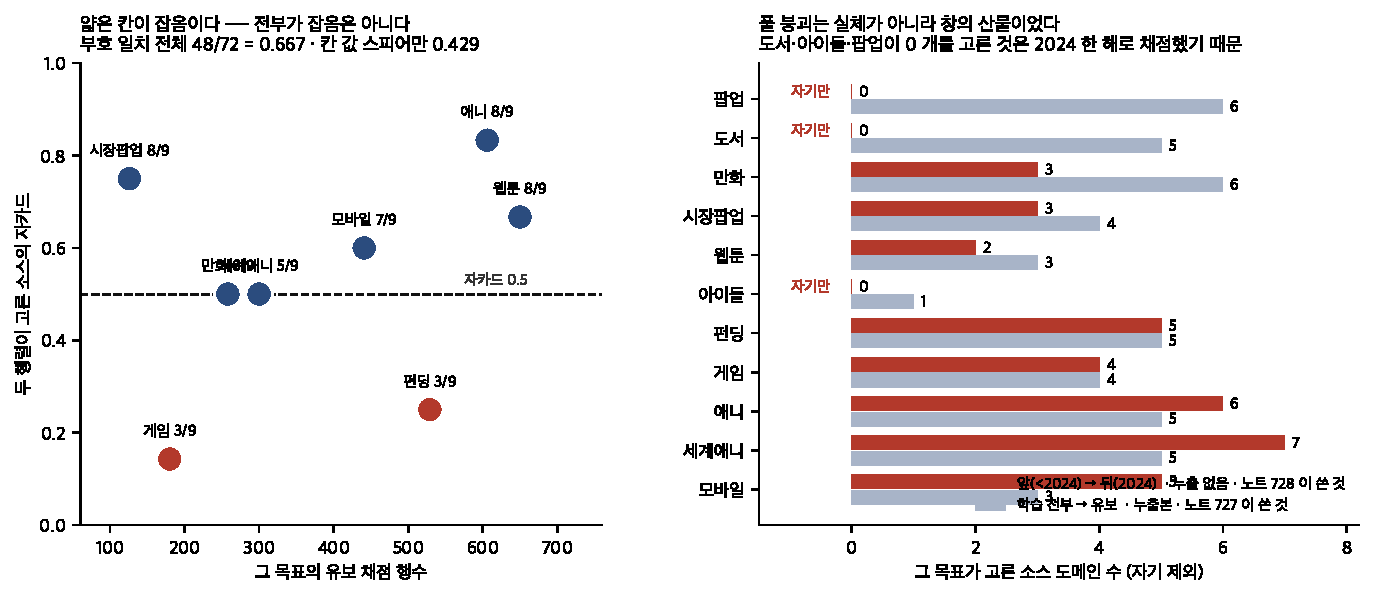
\includegraphics[width=0.99\textwidth]{figs/agree.pdf}
\caption{왼쪽: \textbf{얇은 칸이 잡음이고 전부가 잡음은 아니다} --- 채점 행이 많은
목표에서 두 창이 같은 소스를 고른다(애니 자카드 $0.833$ 대 게임 $0.143$). 오른쪽:
\textbf{풀 붕괴가 실체가 아니라 창의 산물이었다} --- 도서 · 아이돌 · 팝업이 소스를
$0$개 고른 것은 채점을 $2024$ 한 해로 했기 때문이고, 유보로 채점하면 $5$ · $1$ ·
$6$개다.}
\end{figure}

\textbf{그런데 갈리는 \emph{방향}이 법칙과 맞는다.} 자카드가 애니 $0.833$ · 시장팝업
$0.75$ · 웹툰 $0.667$ 인데 \textbf{펀딩 $0.25$ · 게임 $0.143$} 이고, 부호 일치도 같은
순서다($8/9$ 대 $3/9$). \textbf{즉 행렬이 전부 잡음인 것이 아니라 얇은 칸이
잡음이다} --- 노트 717 의 $\text{SD} \propto 1/\sqrt{n}$ 과 같은 방향이다.

\subsection*{그래서 원인 둘이 실은 하나였다}

가장 예상 못 한 결과가 여기 있다. \textbf{누출 없는 앞$\to$뒤 행렬은 도서 · 아이돌 ·
팝업에게 양수 소스를 $0$개 줬다} --- 그래서 그 셋이 자기만 썼고 풀이 무너졌다.
\textbf{같은 절차를 유보로 채점하면 $5$ · $1$ · $6$개다.}

\begin{center}
누출 차단 $\to$ 채점 창이 $2024$ \textbf{한 해}로 줄어듦 $\to$ 행렬 잡음 $\uparrow$
$\to$ 양수 소스 $0$개로 판정 \\
$\to$ \textbf{풀 붕괴}(잡음 $\times 15 \sim 18$) $\to$ 축이 잡음 $\to$
판 신호 몫 $\mathbf{-0.0027}$
\end{center}

\claim{\textbf{노트 729 가 원인을 둘로 적었는데 하나의 사슬이었다.} ``풀을 줄이는
비용''은 독립된 원인이 아니라 \textbf{``고르기 근거가 얇아서 아무것도 못 고른
것''의 결과}다. \textbf{그리고 이것은 누출 차단의 대가다} --- 누출을 막으려면 채점
창을 잘라야 하고, 창을 자르면 고르기 근거가 얇아진다.}
{창을 안 자르고 누출을 막는 길이 있으면 이 서술이 바뀐다 --- 예컨대 앞 구간을
$K$겹으로 갈라 겹마다 채점하면 창을 안 줄이고 행을 늘릴 수 있다. \textbf{그
실험은 안 돌렸다} --- 아래에서 왜 그것으로도 지금 자료에서는 부족한지 적는다.}

\subsection*{유혹적인 후속 실험은 해석이 안 된다 --- 그래서 트랙을 닫는다}

\emph{``누출본 행렬로 고르면 풀이 안 무너지니 판이 오르나''}를 재고 싶어진다.
\textbf{그 측정은 해석 불가다.} 유보로 고르면 유보가 축에 새는데, \textbf{위약 팔은
값을 섞을 뿐 \emph{고르기}의 누출을 지우지 않는다} --- 그러면 신호 몫이 올라도 그것이
전이인지 누출인지 못 가른다.

\claim{\textbf{고르기 추정기의 잡음을 정당하게 줄이는 길은 채점 행을 늘리는 것
하나뿐이고, 그것은 자료가 자라야 한다.} 그러므로 \textbf{T5 는 닫힌 채로 둔다} ---
판 $-0.0027$ 은 이 사슬과 무관하게 측정된 값이고, 사슬을 풀 방법이 지금 없다.}
{앞 구간 $K$겹 채점으로 행을 늘리면 부분적으로 풀린다. 그러나 도서 $80$행 · 아이돌
$56$행에서는 겹을 나눠도 칸이 얇다 --- \textbf{작은 도메인에서는 어떤 절차로도 소스를
못 고른다.} 그것이 자료의 성질이고 배선의 문제가 아니다.}

\section{가장 놀란 것 --- 같은 도메인이 부호를 뒤집었다}

시장팝업 신호 몫이 \textbf{$-0.1191$} 이다. 노트 721(전부 공유)에서는
\textbf{$+0.1857$} 이었고 노트 698 에서는 $+0.1534$ 였다. \textbf{같은 도메인 ·
같은 종류의 축 · 같은 판인데 부호가 뒤집혔다.} 그리고 이번에도 그 도메인이 판을
가장 크게 움직였다(판 기여 $-0.00445$) --- \textbf{방향만 반대다.}

노트 723 이 그 도메인의 축 품질을 $-0.0393$(음수)으로 쟀다. 두 사실을 붙이면 설명이
하나 남는다.

\claim{\textbf{시장팝업의 ``이득''은 처음부터 좋은 예보가 아니라 판이 부호를 뒤집어
쓰던 신호였다.} 축 자체가 라벨과 음의 상관이므로 트리 모형이 그것을 뒤집어 쓸 수
있고, \textbf{축을 바꾸면 그 뒤집기가 안 맞게 된다} --- 그래서 부호가 갈린다.
\textbf{이것은 논문 142 가 세운 조항이 값을 한 이 실험실의 첫 사례다}: \emph{``신호
몫을 보고할 때 그 도메인의 축 품질을 같이 적는다.''}}
{판 안에서 그 열의 쓰임을 직접 보면(분기 기여) 이 설명이 검증된다. 안 봤다.
대안 설명은 ``$126$행 유보라 그냥 잡음''인데, 그 도메인 문턱 $0.0233$ 의 $5$배 밖
값이 세 번 연속 나왔으므로 잡음만으로는 부족하다 --- \textbf{다만 부호가 뒤집힌
것까지 설명하려면 잡음이 아니라 기제가 필요하고, 그 기제를 나는 아직 안 봤다.}}

\section{T5 를 닫는다 --- 문 셋과 그 사이에 알아낸 것}

\begin{center}
\begin{tabular}{llrl}
\toprule
& 문 & 판 신호 몫 & 판정 \\
\midrule
① & 공유 어휘·가중 (노트 698) & $+0.0040$ & 문턱 미달 · 시장팝업 빼면 $-0.0018$ \\
② & 공유 트렁크 $+$ 도메인 임베딩 (721) & $+0.0106$ & 빼면 $+0.0038$ 로 미달 \\
③ & \textbf{소스 고르기} (729) & $\mathbf{-0.0027}$ & \textbf{위약보다 나쁘다} \\
\bottomrule
\end{tabular}
\end{center}

\textbf{배선은 뚫려 있었다.} 임베딩은 도메인을 \emph{가르는} 데 성공했고(코사인
$0.648$ · 붕괴 안 함) 축이 $11/11$ 도메인에 붙었다. \textbf{문제는 나눌 것이
없다는 것이다} --- 전이 행렬이 비대칭이고($a\to b$ 대 $b\to a$ 스피어만 $-0.143$)
\textbf{주는 힘이 열 중 아홉 음수}이며(노트 727) 여덟 도메인에서 LODO 가
음수다(노트 723).

\claim{\textbf{``공유 인코더 $+$ 도메인별 토큰''은 이 자료에서 안 된다 --- 배선이
아니라 자료 때문이다.} 도메인 사이 텍스트$\to$라벨 관계가 크기가 아니라
\textbf{방향까지} 다르다. \textbf{텍스트 표현은 도메인 안 전용으로 확정한다} ---
이것은 노트 719(텍스트 열은 판 안 열)와 같은 방향이다.}
{\textbf{제목만 썼다.} 표현이 얇아서 공유할 것이 없어 보이는 것일 수 있다 --- 줄거리
· 이미지 · 가격 구조 같은 두꺼운 표현이 생기면 같은 절차를 다시 돌려야 한다. 트렁크가
$2{,}497$ 모수라 $121$칸 행렬이 몇 분이므로 \textbf{되돌리는 비용이 싸다.} 그것이 이
트랙을 ``닫힘''으로 적고 ``없음''으로 적지 않은 이유다.}

\section{도구 결함 하나 --- 내가 고치면서 만들었다}

T5 를 닫고 트랙 고르기(\texttt{paper.program next})를 돌렸는데 \textbf{T5 가 여전히
``지금 가능''으로 나왔다.} 원인은 \textbf{상태를 산문에서 추론}한 것이다 ---
\texttt{"대기" in e or "없음" in e}. 내 글은 ``없\emph{다}''였다.

\textbf{그래서 \texttt{"없다"} 를 검사에 더했더니 T7 이 ``막힘''으로 뒤집혔다} ---
T7 의 글에 \emph{``배선은 보류다(둘째 적재가 없다)''}라는 \textbf{곁설명}이 있었기
때문이다.

\claim{\textbf{문자열 검사 결함을 문자열 검사로 고치면 반대편 오탐이 난다.} 그래서
추론을 지우고 \textbf{상태를 값으로 요구}했다(\texttt{\{지금 가능, 막힘, 닫힘,
쉼\}}), 값이 없으면 \texttt{check} 가 규약 위반으로 잡는다. \textbf{제어값을 사람용
산문에서 읽지 않는다} --- 규약 $15$.}
{이 계열이 여섯 번째다(노트 $674$ 부분 문자열 · $677$ 숫자 경계 · $693$ 이름 범위 ·
$697$ 문맥 · $730$ 상태 둘). \textbf{여섯 번 같은 계열이 나왔다는 것은 규율이 아니라
설계로 막아야 한다는 뜻이다} --- 다음은 ``산문에서 값을 읽는 자리''를 감사로 전수
찾는 것이고, 아직 안 했다.}

\subsection*{그리고 노트 729 의 숫자 하나를 정정한다}

이 논문을 쓰려고 풀 크기를 실측했다. \textbf{노트 729 에 도서 $241$행 · 아이돌
$81$행이라 적었는데 실측은 $80$ · $56$ 이다} --- 학습행이 아니라 \textbf{유보까지
더한 수}를 적었다. \textbf{정정 방향이 결론을 강화한다} --- 잡음 배수가 내가 적은
$9$배가 아니라 $\mathbf{15.2}$배 · $\mathbf{18.2}$배다.

\end{document}
